\documentclass[12pt]{article}

% preamble
\usepackage{amsmath}
\usepackage[margin = 1in]{geometry}
\usepackage{graphicx}
\usepackage{booktabs}
\usepackage{natbib}
\usepackage{multirow}
\usepackage{multicol}
\usepackage{setspace}

% highlighting hyper links
\usepackage[colorlinks=true, citecolor=blue]{hyperref}

\title{Comparison of Multi-Class Classification Methods}
\author{Sean Murphy\\
  Statistics Major\\
  University of Connecticut
}

\doublespacing
\begin{document}
\maketitle

\begin{abstract}
THE ABSTRACT WILL BE WRITTEN AFTER THE REST OF THE PAPER HAS BEEN WRITTEN. 
\end{abstract}

\section{Introduction}
\label{sec:intro}

One central facet of the data science/machine learning world is the ability of 
researchers to design models that will accurately predict outcomes based on data.  
Indeed, this is one of the major functions that data scientists play in the 
commercial world, academia, and elsewhere.  There is a tremendous demand, 
especially with the gargantuan quantities of data that are now at our disposal, 
for data scientists who can build effective models to learn from data and make 
accurate predictions for the future.

In general, prediction tasks can be of two types, depending on the characteristics 
of the response variable.  When the variable of interest is a numeric quantity, 
then the prediction task is termed \textit{regression}.  When the variable of 
interest takes different classes, however, the prediction task is termed 
\textit{classification}.  In classification, the goal of the researcher is to build 
a model that learns effectively from the input variables, the \textit{predictors}, 
and spits out accurate predictions of the class that should be assigned for a given 
vector of predictors, $x$.  The researcher considers various different models with 
their own respective strengths and weaknesses, and compares their relative 
performance to select the strongest one. 

Within classification, there are also two distinct types.  The simplest form of 
classification is \textit{binary classification}.  This is the circumstance in 
which the response variable only takes one of two classes, and the task is to 
predict which of these classes a given observation will take.  However, a response 
variable can take more than two classes.  This form of classification is known as 
\textit{multi-class classification}, and results in more complex models.

As there are both many different classification models and many different metrics 
for evaluating the effectiveness of classification models, there has been much 
literature comparing these methods.  Since the classification models all make 
different underlying assumptions, and since they have different relative strengths 
in different circumstances, it is a common practice to compare the performance of 
these methods on different datasets.  Comparisons of multi-class classification 
methods have been carried out by \citep{alsafy2014multiclass}, 
\citep{khan2023comparison}, and \citep{szollHosi2012comparison}.  Additionally, 
there are papers such as \citep{grandini2020metrics} and \citep{grandini2020metrics} 
that compare the utility of different classification metrics, depending upon the 
dataset and its associated characteristics.  

This paper will follow a similar vein of exploring various multi-class 
classification methods by a comparative analysis.  The analysis will focus on a 
dataset containing information on a collection of 1,599 red wine samples from 
northern Portugal.  The goal will be to predict the wine quality from a choice 
of 11 predictors, all of which are numeric physiochemical measurements of the wine 
samples.  I will fit a series of different multi-class classification models to 
the data, and will use several different metrics to comparatively evaluate their 
performance.  From this analysis I hope to deduce which particular features of the 
dataset make it suitable for the classification method that proves the best.  I 
also aim to give an account of why the poorer-performing methods failed to provide 
relatively accurate predictions for the red wine quality.  

The rest of the paper will be organized in the following way.  
An introduction to the red wine data set will be presented in 
Section~\ref{sec:data}.  This section will describe the variables 
and observations contained in the dataset, and will include a brief 
overview of summary statistics.  Next, a methodological overview of 
this analysis will be given in Section~\ref{sec:meth}.  Each of the 
classification methods and their underlying assumptions will be 
presented in Section~\ref{sec:class}.  The classification metrics 
which will be used to compare the predictive effectiveness of each 
model will be introduced in Section~\ref{sec:metr}.  After this, 
the results will be presented with tables and figures in 
Section~\ref{sec:resu}.  Finally, once the results of the analysis 
have been described, a discussion of their implications and 
suggestions for further study will be covered in Section~\ref{sec:disc}.


\section{Data}
\label{sec:data}

The data that will be analyzed in this study comes from the UC Irvine Machine 
Learning Repository.  It is a dataset from 2009 containing information about 
a sample of red "Vinho Verde" wine from north Portugal.  The dataset contains 
$n = 1,599$ observations (different wine samples) of twelve variables, eleven 
of which are continuous numeric variables.  These continuous variables are 
different physiochemical measurements of the wine samples: fixed acidity, 
volatile acidity, citric acid, residual sugar, chlorides, free sulfur dioxide, 
total sulfur dioxide, density, pH, sulfates and alcohol.  The other variable 
contained in the dataset is wine quality, which takes integer values from 0-10 
(0 being lowest quality, 10 being highest quality).  Though numeric, this 
variable will be treated as having 11 classes, and will be the response 
variable in the analysis.  The goal is to predict the class of wine quality 
for a given sample of red wine based on its physiochemical properties.  

One important note before describing the methodology of this study concerns the 
response variable, wine quality.  A boxplot and histogram of the distribution of 
observations according to their wine quality levels can be seen in 
Figure~\ref{fig:wine}.  We can see that there are no wine samples in our dataset 
that had quality levels of 0, 1, 2, 9, or 10.  All of the quality levels fell 
within the range from 3 to 8, and within this range, the vast majority were rated 
either a 5 or a 6.  Indeed, these two levels alone account for over 82 percent of 
the data.  We can see in the histogram and boxplot in Figure~\ref{fig:wine} that 
the distribution of wine quality levels is roughly symmetric, with outliers 
depicted in the boxplot at quality levels of 3 and 8.  Thus, the response variable 
has unbalanced classes; there are far from an equal number of observations in each 
class, especially considering that some classes do not contain any observations.  
The models built in this analysis will consequently ignore the missing classes for 
which there are no training observations.  

\begin{figure}[tbp]
 \centering
 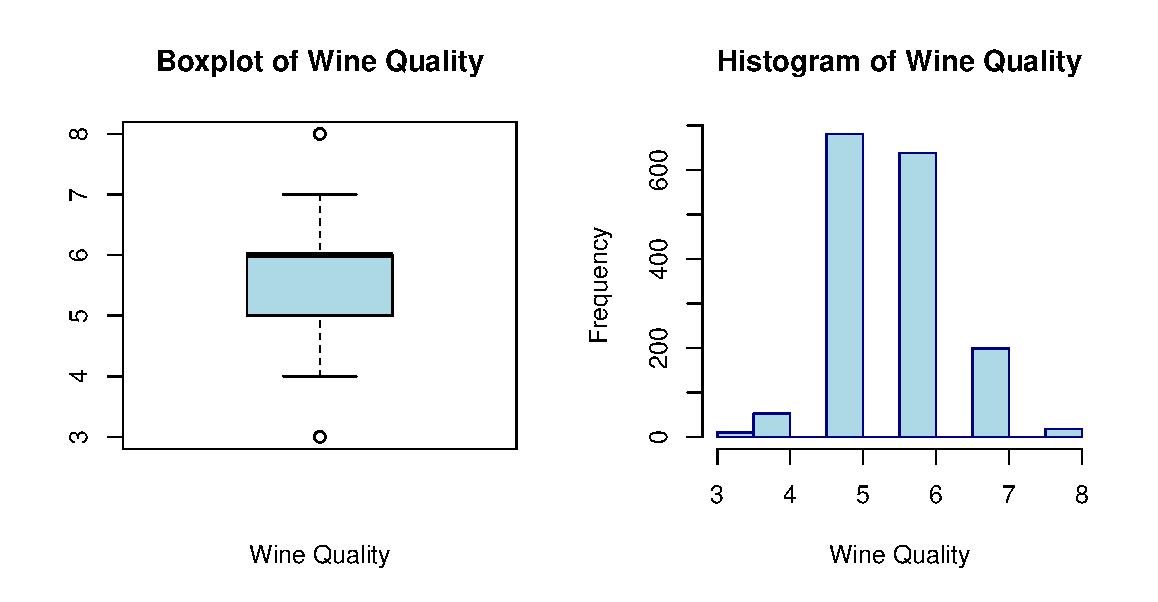
\includegraphics[width=\textwidth]{manuscriptfigure.pdf}
 \caption{A boxplot and a histogram of the wine quality for the samples of Portuguese red wine.}
 \label{fig:wine}
\end{figure}

\section{Methods}
\label{sec:meth}

OVERVIEW PARAGRAPH

Before proceeding straight into the analysis, it is necessary first to give an 
overview of the methodology that will be employed.  That means, first, summarizing 
how the data will be prepared, then introducing the models that will be used for 
this analysis.  Finally, this section will also introduce the various metrics that 
will be used to evaluate model performance and to select the best classification 
method for the given dataset.  

\subsection{Data Preparation}
\label{sec:prep}

Fortunately, the red wine dataset is quite clean.  In the 1,599 rows of the data 
frame, there are no NA values, and thus no rows have to be removed.  

In order to be able to fit various models to the data set, we will first divide the 
dataset into a training and a test set.  The training set will comprise roughly half 
the dataset, and will be used to train the models, as the name would suggest.  Thus, 
it is from the data in the training set that the models will be constructed.  
Observations from the red wine dataset will be assigned to the training set randomly, 
to avoid any kind of bias that would result from non-random training set selection.  

The other half of the dataset will contain the test set.  The test set will be used to 
test the predictive accuracy of the models that were fitted using the training data.  
The fitted models will take as input the predictor values in the test set, and will 
spit out predictions for the response variable corresponding to each observation.  
These classification predictions will then be compared to the observed response variable 
classes for each observation.  From this comparison, the overall accuracy of each model 
can be discerned, and they can be compared based on these findings.  The model that 
proves to perform the best will be the model that has the greatest overall prediction 
accuracy, and this is the model that will be recommended for use. 


\subsection{Classification Methods}
\label{sec:class}

\subsubsection{Generative Models}
\label{sec:gm}

OVERVIEW PARAGRAPH

The next three multi-class classification methods are very similar in structure, 
and so it will be useful to introduce their shared underlying methodology before 
discussing their peculiarities.  In multinomial logistic regression, the approach 
is to attempt to model $Pr( Y = k|X = x)$ directly.  However, there is an 
alternative approach that can prove more useful in certain circumstances.  This 
approach is to employ Bayes' Theorem, which obtains $Pr( Y = k | X = x)$ indirectly 
by first obtaining the conditional distribution of $X$ in each class, $K$, and then 
using these distributions to obtain the desired probability that $Y$ will fall into 
$k$ given some vector of predictors $x$.  The general model takes the following form:
\begin{equation}
  \label{eq:genmod}
  Pr(Y = k | X = x) =
  \frac{\pi_k f_k(x)} {\sum_{l = 1} ^ {K} \pi_l f_l(x)}
\end{equation}
In Equation~\eqref{eq:genmod}, the $\pi_k$ term in the numerator simply is the prior 
probability that $Y$ falls into class $k$.  This is computed by the proportion of all 
the observations in the sample that fall into the $k ^ {th}$ class.  The $f_k(x)$ term 
describes the conditional distribution of $X$ in class $k$.  In other words, 
$f_k(x) = Pr(X = x | Y = k)$.  These two numerator terms are divided by the same two 
terms for each class $k$ summed in the denominator.  That is, the denominator contains 
the sum of the prior probabilities that $Y$ will fall into each of the $K$ classes 
multiplied by the corresponding conditional distribution of $X$ in that class.  Thus, 
the general form of the generative model is simply Bayes' Theorem, which returns here 
an estimate of the probability that $Y$ will fall into class $k$ given some vector of 
predictors.  

Each of the next three multi-class classification models that we will consider is some 
variant of the above, and they are principally differentiated by their varying strategies 
for approximating $f_k(x)$.  The three kinds of generative models that we will consider 
in this paper are linear discriminant analysis (LDA), quadratic discriminant analysis 
(QDA), and naive Bayes (NB).  We will discuss each of them in turn.  

LINEAR DISCRIMINANT ANALYSIS

Linear Discriminant Analysis (LDA) is a generative model that approximates $f_k(x)$ by 
assuming that each of the predictors comes from a normal distribution.  In the case of 
multiple predictors such as we have in this analysis, this means that LDA assumes $x$ 
(the vector of $p$ predictors) follows a multivariate normal distribution.  The mean, 
$\mu$, of this multivariate normal distribution is a vector containing the mean value 
of each predictor.  The covariance of the predictors, $\Sigma$, is the $p$ by $p$ 
covariance matrix of the vector $x$.  Therefore, we can say in shorthand that 
$x ~ N(\mu,\Sigma)$.  Thus, since the conditional distribution of the vector $x$ in 
each class $k$ is assumed to be multivariate normal, the density function is 
$$Pr(X = x|Y = k) = \frac {1} {(2\pi) ^ {p/2} |\Sigma| ^ 
{1/2}} exp(-\frac{1}{2}   (x - \mu_k) ^ T \Sigma ^ {-1} (x - \mu_k))$$.  
Here, $\mu_k$ is simply the vector of the mean values of the $p$ predictors where 
$Y = k$, and $\Sigma$ is the common covariance matrix of $x$ for each of the $k$ 
classes.  The above equation can then be plugged into Equation~\eqref{eq:genmod} 
for $f_k(x)$, the resulting equation of which we will not reproduce here because of 
its complexity.  Suffice it to say that this equation now obtains for us the probability 
that $Y$ falls in class $k$ given a particular vector of predictors $x$, so that the 
model gives the value for $Pr(Y = k|X = x)$.

In order to classify a vector of predictors $x$ to some class $Y = k$, we look for the 
class in which the value of the above $Pr(Y = k|X = x)$ is greatest.  With some 
algebraic rearrangement, this is equivalent to classifying a vector $x$ to the 
class for which the following equation is greatest:
\begin{equation}
  \label{eq:disscore}
  \delta_k(x) = x ^ T \Sigma ^ {-1} \mu_k - 
  \frac {1} {2} \mu_k ^ T \Sigma ^ {-1} \mu_k + \log {\pi_k}
\end{equation}. 

Equation~\eqref{eq:disscore} is called the \textit{discriminant score}.  If a class 
has the greatest value of $\delta_k(x)$ for some vector of predictors $x$, then that 
vector of predictors will be classified to the corresponding class. Linear 
discriminant analysis gets its name from the fact that this discriminant score is a 
linear function of $x$. 

In Equation~\eqref{eq:disscore}, each $\mu_k$ is estimated by combining the mean value 
for each predictor in the sample into a vector, $\hat{\mu_k}$.  The values of $\pi_k$ 
are once again the prior probability that $Y$ falls into class $k$, calculated by the 
proportion of the total observations in class $k$.  Finally, the covariance matrix of 
the predictors, $\Sigma$, is estimated by finding the covariance matrix of the 
predictors in the sample. 

NAIVE Bayes

Naive Bayes (NB) is distinct from LDA and QDA in the manner it estimates $f_k(x)$, 
the conditional joint distribution of the $p$ predictors given that $Y$ is in some 
class $k$.  Whereas LDA and QDA both assume that this joint distribution is a multivariate 
normal distribution, NB assumes that each of the $p$ predictors are independent within each 
class.  Thus, for a particular class, the joint probability distribution of all the 
predictors given that $Y$ falls in that class is simply a product of the individual densities 
of each of the predictors given $Y = k$.  In more formal terms, because of this assumption of 
the independence of each predictor within each class, NB estimates $f_k(x)$ in the following 
manner:
\begin{equation}
  \label{eq:indprob}
  f_k(x) = f_{k1}(x_1) \times f_{k2}(x_2) \times ... \times f_{kp}(x_p)
\end{equation} 
where $k = 1, 2, ..., K$, and $x_1, x_2, ..., x_p$ are the $p$ predictors in the training set.  
Thus, Equation~\eqref{eq:indprob} can simply be plugged into Equation~\eqref{eq:genmod} for 
$f_k(x)$ in the following manner:
\begin{equation}
  \label{eq:nb}
   Pr(Y = k | X = x) =
  \frac{\pi_k [f_{k1}(x_1) \times f_{k2}(x_2) \times ... \times f_{kp}(x_p)]} 
  {\sum_{l = 1} ^ {K} \pi_l [f_{l1}(x_1) \times f_{l2}(x_2) \times ... \times f_{lp}(x_p)]}
\end{equation} 
where $k = 1, 2, ..., K$.  The $f_{kp}(x_p)$ terms in Equation~\eqref{eq:nb} are much simpler 
to estimate than the joint distribution of each of the predictors, so NB simplifies the 
analysis greatly.  Though there are many strategies for estimating these individual predictor 
densities within each class, these strategies will not be covered within this paper.  

Although NB makes a strong (and often in practice, untrue) assumption about the independence 
of the predictors, it still performs quite well in many circumstances.  It is particularly 
well suited to situations in which the training set is not large enough relative to the 
number of predictors to effectively estimate the joint density of each of the predictors.  

K NEAREST NEIGHBORS

The K Nearest Neighbors (KNN) approach to multi-class classification is markedly different 
from those covered previously.  It has a rather intuitive design, and its methodology is 
rather straightforward.  Interestingly enough, it also often obtains usefully low test 
error rates and can perform quite well on many data sets.  

Up until now, $K$ has signified the number of distinct classes that can be taken by $Y$, 
the response variable of interest.  In KNN, K refers to the number of nearest neighbors 
upon which the classification prediction is based.  To forestall further confusion, 
therefore, $K$ will still be used to denote the number of classes taken by $Y$, while 
$K ^ *$ will refer to the number of nearest neighbors in KNN analysis.  

The basic idea behind KNN is that, if we wish to accurately predict which class $Y$ will 
fall into given some vector of predictors $x$, we ought simply to look at the classes 
taken by $Y$ given vectors as similar to $x$ as we can find in our dataset.  In practical 
terms, this means that we base our prediction of $Y$'s class upon the class taken by the 
largest number of the $K ^ *$ nearest neighbors to $x$.  The $K ^ *$ nearest neighbor 
observations to $x$ are the observations with the shortest Euclidean distance to the 
vector $x$.  The value of $K ^ *$ can be adjusted by the researcher when fitting KNN 
models, since different values of $K ^ *$ will perform better under different scenarios.  
Thus, one can fit many different KNN models to the same dataset, each with different 
numbers of nearest neighbors, to predict the class of $Y$ for some vector of predictors, 
$x$.  

One notable drawback of KNN analysis is its decreased accuracy as the number of 
predictors increases.  Holding all other things constant, when the number of predictors 
increases, the Euclidean distance between the vector $x$ of interest and each of its 
$K ^ *$ nearest neighbors also increases.  As such, the nearest neighbors to $x$ provide 
decreasingly satisfactory approximations of $x$, and thus KNN models fitted in high 
dimensions (i.e., with many predictors) tend to have poorer performance in terms of 
prediction accuracy and test errors.  This pattern is known as the 
\textit{curse of dimensionality}, and is an important reason to be wary in instances of 
large values of $p$.  Fortunately, for this present analysis, $p = 11$ is relatively 
small. 

SUPPORT VECTOR MACHINES

\subsection{Classification Metrics}
\label{sec:metr}

OVERVIEW PARAGRAPH

Once the models have been constructed, the next task is to select the criteria 
by which their performance will be evaluated and compared.  As it turns out, 
when it comes to multi-class classification problems, there are many ways to 
accomplish this task, and the analyst must select the method that is best 
suited to their purposes.  Without going into an excessive degree of length, 
this section will present a brief overview of some of the simpler methods of 
analyzing model performance.  Each of the metrics surveyed here depend upon 
the more basic notion of a confusion matrix, which will be discussed first.  
Then, the subsequent discussion will focus on the calculations that can be 
made with confusion matrices as their foundation, as well as the situations 
in which they are more or less appropriate.  Ultimately, two of these metrics 
will be used for the analysis in this paper: the overall Classification 
Accuracy Value, and the Weighted Balanced Accuracy.   

CONFUSION MATRICES

A confusion matrix is a basic analytical tool for evaluating classification model performance.  

MAKE A CONFUSION MATRIX HERE
\begin{table}[tbp]
\caption{This is a hypothetical example of a multi-class confusion matrix.}
\label{tab:conf}
\centering
\begin{tabular}{ |p{3cm}||p{3cm}|p{3cm}|p{3cm}|  }
 \hline
 \multicolumn{4}{|c|}{Country List} \\
 \hline
 Afghanistan   & AF    &AFG&   004\\
 Aland Islands&   AX  & ALA   &248\\
 Albania &AL & ALB&  008\\
 Algeria    &DZ & DZA&  012\\
 American Samoa&   AS  & ASM&016\\
 Andorra& AD  & AND   &020\\
 Angola& AO  & AGO&024\\
 \hline
\end{tabular}
\end{table}

In the confusion matrix in Table~\ref{tab:conf}, the predicted classes are the 
rows and the actual (test dataset) classes are the columns.  The classes in 
both the rows and columns are presented in exactly the same order.  Thus, when 
the model predicts that a particular observation will take on a specific class, 
if that same observation took the predicted class in the test dataset, then the 
row and column values match.  This would be an instance of an observation that 
is correctly predicted by the model.  Thus, since the classes in the rows and 
columns are presented in the same order, the diagonal elements of the confusion 
matrix are the correctly predicted observations.  These are all the observations 
whose predicted class matches its actual class.  

On the other hand, all the elements of the confusion matrix that are not on the 
diagonal are the incorrectly predicted observations.  These are the observations 
whose predicted class does not match their actual class.  The calculations in 
the metrics that follow are predicated on the presentation of correctly versus 
incorrectly predicted observations in the confusion matrix.  

CLASSIFICATION ACCURACY VALUE

The Classification Accuracy Value (CAV) is the simplest and most straightforward 
means of assessing the overall prediction accuracy of a classification model.  To 
calculate the CAV using a confusion matrix, simply sum the diagonal elements of 
the matrix in the numerator, and sum all the elements of the matrix in the 
denominator.  The corresponding proportion will be the proportion of observations 
whose class is predicted accurately by the model.  This value is the Classification 
Accuracy Value.  The calculation for this metric is presented in 
Equation~\eqref{eq:cav}:
\begin{equation}
    \label{eq:cav}
    CAV = \frac {T} {T + F}
\end{equation}
, where $T$ stands for the true predictions (on the diagonal of the matrix) and $F$ 
stands for the false predictions, which are the non-diagonal elements.  

The CAV is best applied in situations where the overall prediction accuracy of the 
model is of the highest concern, and where class-specific prediction accuracy is less 
important.  In terms of the CAV, each observation is equally weighted, but the 
relative prediction accuracy within each class is not taken as strictly into account 
as in other metrics, as we shall see below.  If it is of the utmost importance that 
the model has a high prediction accuracy for each class, then other metrics may be 
applied that take this factor into account.

BALANCED ACCURACY VALUE

In order to have a metric that takes into account the class-specific prediction 
accuracy of the model, a slight modification must be made to the formula in 
Equation~\eqref{eq:cav}.  The modification in this case will weight the prediction 
accuracy for each class equally, so that the prediction accuracy of the classes 
containing the most observations does not dominate the accuracy metric.  The 
modification will be made in the following way:
\begin{equation}
    \label{eq:bav}
    BAV = \frac {\Sigma_ {k=1} ^ {K} \frac {T_k} {n_k}} {K}
\end{equation}
, where K denotes the number of classes taken by the response variable.  

In Equation~\eqref{eq:bav}, BAV stands for the Balanced Accuracy Value.  In the 
numerator, $T_k$ stands for the number of true predictions in class $k$.  That 
is to say, it is the number of observations in class $k$ that were predicted to 
take class $k$ by the model.  Within a column, this will be the value that falls 
on the diagonal of the matrix.  In Equation~\eqref{eq:bav}, the $n_k$ term denotes 
the total number of observations falling in the $k^{th}$ class.  Thus, each fraction 
that is summed in the numerator is simply the prediction accuracy within the $k^{th}$ 
class.  This means that the equation itself simply returns the average of the 
prediction accuracy values within each class.  The equation calculates the proportion 
of the observations within each class that were predicted accurately, sums these 
values for each of the $1...K$ classes, and then divides the $K$ classes to return 
the average value.

This metric is best employed in situations where it is highly important for the model 
to predict each class accurately.  Some models may predict certain classes far better 
than they do other classes.  Such models will be penalized in their BAV ratings, 
because the classes for which model prediction accuracy suffers will draw the BAV 
level down. 

It is important to note one substantial qualification on the preceding paragraph.  
The BAV equation necessitates that each class's prediction accuracy will be weighted 
exactly the same as the others.  This is because what is being summed in the numerator 
are fractions, that are all $\geq 0$ and $\leq 1$ regardless of how many observations 
from the dataset actually fell into that category.  When each class has roughly the 
same amount of observations, the dataset is said to be \textit{balanced}, while 
datasets with varying observation amounts per class are said to be \textit{unbalanced}.  
In the case of a balanced dataset, the BAV value will not differ greatly at all from 
the CAV value.  In fact, if the dataset is perfectly balanced, the two values will be 
identical \citep{grandini2020metrics}.  This is because the effect of equalizing the 
weights of each class in the BAV is negligible when each class does actually have the 
same weight in the dataset.

On the other hand, BAV values differ substantially from CAV values when the dataset is 
heavily unbalanced and there are significant disparities between the class-specific 
prediction accuracy of many of the classes.  In a situation such as this, the 
researcher may determine it wise to employ BAV if it is important to predict each 
class accurately to get a more fitting evaluation of the model's appropriateness for 
subsequent predictions.  

\section{Results}
\label{sec:resu}

OVERVIEW PARAGRAPH

OPTIONAL: PRESENT CONFUSION MATRICES FOR EACH OF THE METHODS

PRESENT ACC VALUES FOR EACH OF THE METHODS IN COMPARATIVE CHART

PRESENT ROC CURVES FOR EACH OF THE METHODS

PRESENT AUC VALUES FOR EACH OF THE METHODS IN COMPARATIVE CHART

\section{Discussion}
\label{sec:disc}

% What are the main contributions again?

% What are the limitations of this study?

% What are worth pursuing further in the future?

% Watch for prevalence of diabetes \citep{wild2004global}.

\bibliography{references}
\bibliographystyle{chicago}

\end{document}